\section{Localized bridges, recoverable cuts, and length moments}
\label{sec:08-sewing-renewal}

We first seek a positive chance of a long bridge that remains in a box
of size comparable to its height. Fix its bottom source port. For a fixed
confinement constant $C$, write
\[
 m_i(h)=\sum_{\substack{\gamma\text{ strict bridge of height }h\\
                         \operatorname{diam}\gamma\le Ch}}
              \rho^{|\gamma|}|\gamma|^i.
\]
Our first goal is to choose $C$ so that
\[
 m_1(h)\ge h^{13/12-o(1)},\qquad
 m_2(h)\le h^{29/12+o(1)}.
\]
Together with $m_0(h)\le B_h\asymp h^{-1/4}$, these estimates will give
subpower probability of length at least $h^{4/3-\xi}$ for every fixed
$\xi>0$. Section~\ref{sec:renewal} will amplify that probability.

The two moments come from different constructions. To bound $m_2$, we
close a confined path outside its strip and use the polygon length-square
estimate. To bound $m_1$ below, we begin with the bulk length supplied by
the nesting comparison and attach exterior paths to make a bridge.
Both constructions require localized path mass and a way to recover the
sewing lines from their output. We develop those tools first, using the
port and band conventions of Section~\ref{sec:inputs}. All sums below are
unnormalized critical masses.

After establishing the length estimate, the final subsection proves a
second geometric fact needed for the ordered adjacent paths in
Section~\ref{sec:10-thermal-probes}: a path can turn around an obstacle
with a free terminal port while retaining mass at least $cH^{-1/4}$.
That construction needs the exact power, without exponent slack, and
uses a second moment of its representations.

\subsection{Localization and recoverable seams}

\begin{lemma}[Convex cuts and lateral localization]
\label{lem:08-localization}
In a convex lattice domain, removing the part beyond a lattice cut compares
the mass of old boundary exits lost with the mass of exits on the new cut,
up to absolute positive constants. In particular, paths from a side which
reach a parallel cut \(r\) bands away have boundary-exit mass at most
\(C B_r\). In a strip of height \(h\), the arch or bridge mass from a fixed
bottom port lost by requiring lateral extent at most \(M\) is at most
\[
 C h M^{-5/4},\qquad M\ge C_1h.
\]
\end{lemma}
\begin{proof}
Take real parts in the boundary winding identity before and after making
the cut. Contributions of paths contained in the near subdomain cancel.
For every other boundary exit the cosine is between the same positive
constant and one, since both domains are convex. Thus the lost old exit
mass and the new-cut exit mass are comparable. For a parallel cut, its
exits are a subset of the bridges across the intervening strip. This also
explains the lower comparison used later: a family of paths in the old
domain which necessarily passes the cut gives a lower bound, up to a
constant, for the mass of exits on that cut. No bound on the continuation
of an individual prefix is required.

For localization truncate the strip to a parallelogram whose width is a
small fixed multiple of \(M\), and average the winding comparison over
bottom sources in its central half. There are \(\asymp M\) such sources.
Reverse paths from a side exit to one of these sources. For each side port
they reach a cut parallel to that side at distance at least \(cM\), so their
total mass is at most \(C B_{\lfloor cM\rfloor}\). There are \(O(h)\)
side ports. The average loss is therefore at most
\(C h M^{-1}B_{\lfloor cM\rfloor}\le C hM^{-5/4}\).
If \(M/h\) is sufficiently large, the parallelogram lies within lateral
distance \(M\) of every central source. For each such source, exceeding
lateral distance $M$ requires leaving this parallelogram. The former mass
is the same for all these sources by translation invariance, so it is
bounded by the average exit loss.
Infinite strips are obtained by increasing finite truncations.
\end{proof}

\begin{lemma}[Variation of the bridge kernel]
\label{lem:08-variation}
With consecutive top ports identified by their tangential coordinates,
\[
 \sum_x|b_h(x+1)-b_h(x)|\le C(B_h-B_{h+1}).
\]
\end{lemma}
\begin{proof}
Put \(\lambda=\pi/8\). Add the two adjacent rhombi shown in
Figure~\ref{fig:08-kernel-bump} above ports $a=x$ and $b=x+1$.
Each rhombus consists of two ordinary triangles. Their four new dual
vertices form the chain $u_0,v_0,u_1,v_1$, with $a$ incident to $u_0$
and $b$ incident to $u_1$. Denote the left and right step exits by $L,R$.
The horizontal top exits have winding zero, while $L$ and $R$ have
windings $+\pi/3$ and $-2\pi/3$, respectively: closing to the source
along the exterior boundary determines these turns.

\begin{figure}[b]
\centering
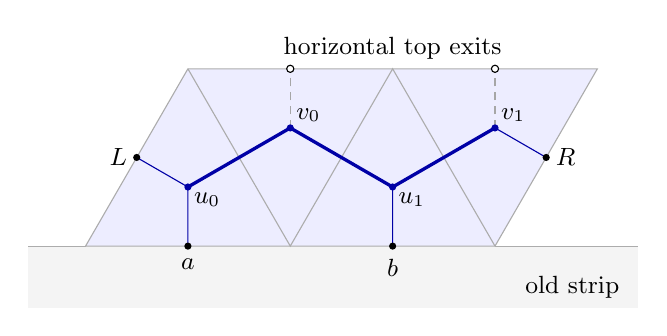
\begin{tikzpicture}[x=2.6cm,y=2.6cm,font=\small]
 \def\d{0.8660254038}
 \fill[gray!9] (-.78,-.30) rectangle (2.20,0);
 \fill[blue!7] (-.5,0)--(1.5,0)--(2,\d)--(0,\d)--cycle;
 \draw[gray!65] (-.5,0)--(1.5,0)--(2,\d)--(0,\d)--cycle;
 \draw[gray!65] (0,\d)--(.5,0)--(1,\d)--(1.5,0);
 \draw[gray!65] (-.78,0)--(-.5,0) (1.5,0)--(2.20,0);
 \draw[very thick,blue!65!black]
    (0,{\d/3})--(.5,{2*\d/3})--(1,{\d/3})--(1.5,{2*\d/3});
 \draw[blue!65!black]
    (0,0)--(0,{\d/3})--(-.25,{\d/2})
    (1,0)--(1,{\d/3})
    (1.5,{2*\d/3})--(1.75,{\d/2});
 \draw[densely dashed,gray!70]
    (.5,{2*\d/3})--(.5,\d)
    (1.5,{2*\d/3})--(1.5,\d);
 \foreach \x/\y/\lab in {0/{\d/3}/u_0,.5/{2*\d/3}/v_0,1/{\d/3}/u_1,1.5/{2*\d/3}/v_1}{
    \fill[blue!65!black] (\x,\y) circle (1.3pt);
 }
 \node[below right,inner sep=2pt] at (0,{\d/3}) {$u_0$};
 \node[above right,inner sep=2pt] at (.5,{2*\d/3}) {$v_0$};
 \node[below right,inner sep=2pt] at (1,{\d/3}) {$u_1$};
 \node[above right,inner sep=2pt] at (1.5,{2*\d/3}) {$v_1$};
 \foreach \x/\lab in {0/a,1/b}{
    \fill (\x,0) circle (1.3pt);
    \node[below] at (\x,-.015) {$\lab$};
 }
 \fill (-.25,{\d/2}) circle (1.3pt);
 \fill (1.75,{\d/2}) circle (1.3pt);
 \node[left] at (-.25,{\d/2}) {$L$};
 \node[right] at (1.75,{\d/2}) {$R$};
 \draw[fill=white] (.5,\d) circle (1.3pt) (1.5,\d) circle (1.3pt);
 \node[above] at (1,\d) {horizontal top exits};
 \node[anchor=west] at (1.60,-.20) {old strip};
\end{tikzpicture}
\caption{The exact two-rhombus addition for the kernel variation.
The four blue vertices are triangle centers; $a,b$ are the old top
ports. A path to $L$ or $R$ enters this chain through exactly one of
$a,b$. The dashed half-edges lead to horizontal exits, whose imaginary
contributions vanish.}
\label{fig:08-kernel-bump}
\end{figure}

A path to $L$ or $R$ crosses the two-port interface an odd number of
times, hence exactly once. The four possible continuations have weights
\[
\begin{array}{c|cc}
 & L & R\\ \hline
 a & \rho & \rho^4\\
 b & \rho^3 & \rho^2
\end{array}
\]
according to the number of new vertices they visit. Thus their combined
contribution to the imaginary identity is
\[
 \sin\lambda\bigl(\rho b_h(x)+\rho^3b_h(x+1)\bigr)
 -\sin(2\lambda)\bigl(\rho^4b_h(x)+\rho^2b_h(x+1)\bigr).
\]
Using $\sin\lambda\,\rho=\sin(2\lambda)\rho^2$, this equals
\[
 \sin\lambda\,\rho(1-\rho^2)
       \bigl(b_h(x)-b_h(x+1)\bigr).
\]
There can be no other occupied segment in the raised part: another visit
would require at least three interface crossings, while its horizontal
top ports are vacant for a path ending at a step exit.

Subtract the old imaginary winding identity. The absolute value of the
remaining bottom contribution is bounded by a constant times the mass of
new arches using the bump. For distinct bump positions these arch families
are disjoint: a member enters and leaves the last band through that specific
adjacent pair, and uses no other port there. Their sum is bounded by
\(A_{h+1}-A_h\). The real strip identity
\(\cos(3\lambda)A_h+B_h=1\), with \(\lambda=\pi/8\), gives
the assertion. To justify the infinite-strip identities, first fix a finite set of
bump positions and perform each calculation in a wide finite
parallelogram. Lemma~\ref{lem:08-localization} bounds every side-error
mass by \(C_h M^{-5/4}\), which tends to zero as the lateral cutoff
\(M\) increases with \(h\) fixed. After this limit, increase the finite
set of bump positions. The nonnegative, disjoint new-arch masses sum
monotonically to at most \(A_{h+1}-A_h\), whose
finiteness is part of Theorem~\ref{thm:01-strip}.
\end{proof}

A \emph{seam} is a lattice line with a specified crossing property that
allows the pieces of a sewn path to be recovered. There is no tangency
convention to choose: a visited internal port is traversed normally, and
crossing a lattice line means traversing such a port. A line crossed once
splits a bridge into two bridges. A line crossed twice, with both endpoints
on its near side, cuts off one arch excursion. Excursions beyond ordered
lines of the latter kind are nested.

\begin{lemma}[Seam moment bounds]
\label{lem:08-seam-moments}
Let $\mathcal F$ be a family of port paths, and let $N(\gamma)$ count
specified seams in an interval of $R$ parallel lattice levels. They are
either once-crossed levels, or twice-crossed levels with both endpoints
on their near side; in the latter case the excursions beyond the counted
levels are nested. Suppose that, after cutting at any ordered list of
such seams, the end pieces have bounded strip or convex boundary sums
when summed successively from their cut ports. Allow a factor $R_0^C$
for source and placement choices, where $C$ is independent of the number
of selected seams and $R\le C_0R_0$.
Then, for every fixed positive integer $j$, the weighted count over
$\mathcal F$ satisfies
\[
 \sum_\gamma\rho^{|\gamma|}N(\gamma)^j
 \le R_0^C C_j
 \begin{cases}
 R^{1+3(j-1)/4},&\text{one crossing},\\
 R^{1+(j-1)/2},&\text{one arch excursion}.
 \end{cases}
\]
Consequently counts exceeding \(R^{3/4}R_0^\varepsilon\), respectively
\(R^{1/2}R_0^\varepsilon\), have arbitrarily polynomially small weighted
mass as \(R_0\to\infty\), including after multiplication by any fixed
polynomial in \(R_0\).
\end{lemma}
\begin{proof}
Expand \(N^j\) and order the selected levels, allowing repetitions. Each
internal gap \(g\) requires one bridge in the first case and two in the
second. Removing mutual avoidance can only increase the resulting upper
bound. The gap factors are therefore at most
\(C(1+g)^{-1/4}\) and \(C(1+g)^{-1/2}\), respectively. Summing the
first level in \(R\) ways and each following gap gives the displayed
bounds, with the ordering and repetitions absorbed in \(C_j\).
For a threshold \(Q\), use
\[
 \sum\rho^{|\gamma|}N^a\mathbf1_{\{N>Q\}}
 \le Q^{-(j-a)}\sum\rho^{|\gamma|}N^j
\]
for a fixed \(a\) and then choose \(j\) sufficiently large. All paths in
a box of diameter \(O(R_0)\) have length \(O(R_0^2)\), so length powers
and raw geometric multiplicities can be included in the polynomial factor.
\end{proof}

This is a statement about an unnormalized weighted measure. Each subsequent
use specifies the end pieces; no probability estimate is inferred merely
by calling a sewing level typical. For a nonnegative representation count
\(F\), we also use the elementary weighted Cauchy--Schwarz inequality
\[
 \sum_{F>0}\rho^{|\gamma|}
 \ge\frac{\bigl(\sum\rho^{|\gamma|}F\bigr)^2}
           {\sum\rho^{|\gamma|}F^2}.
\]

We will also use the two-crossing argument for polygons of bounded
diameter, modulo translation. Choose an extreme counted line and one
crossing port, including these polynomially many choices in the placement
factor. Cutting there makes two port arches. The outer arch has bounded
strip mass, while further counted lines in the other arch produce the
pairs of bridge gaps above. This reduces the polygon count to the same
path calculation without introducing an unrestricted root sum.

\subsection{Prescribed and free endpoints in narrow tubes}

\begin{lemma}[Fixed endpoints in thin tubes]
\label{lem:08-fixed-tube}
There is \(v>0\) such that, for every fixed \(\delta>0\), every attainable
endpoint displacement \(|x|\le vh\) has bridge mass at least
\(h^{-5/4-o(1)}\) in a tube of transverse radius \(\delta h\) about its
straight join. The estimate is uniform in the endpoint and large \(h\).
\end{lemma}
\begin{proof}
We first allow a sufficiently large fixed tube radius. Let \(H\) be even,
choose \(|k-H/4|\le H/40\), and write \(l=H/2-k\).
Lemma~\ref{lem:08-variation}, summed over these heights, implies that a
positive fraction of the choices have both kernel variations at most
\(C H^{-5/4}\). Their suprema have the same bound, since each summable
kernel tends to zero at infinity. Reflection gives \(b_k(x)=b_k(-x)\),
and likewise for \(l\).

For either good kernel \(f\), localization leaves mass \(\ge cH^{-1/4}\)
on \(O(H)\) endpoint positions. Thus
\(\sum f(x)^2\ge cH^{-3/2}\). Moreover
\[
 \left|\sum_x f(x)f(x+t)-\sum_x f(x)^2\right|
 \le \|f\|_\infty\,\|f(\cdot+t)-f\|_1
 \le C|t|H^{-5/2}.
\]
For \(|t|\le v_0H\), with \(v_0>0\) sufficiently small, the
correlation is at least \(c'H^{-3/2}\). Symmetry turns this into the same
lower bound for the self-convolution. If both constituent bridges are
confined to a lateral box of radius \(DH\), the convolution loss is at
most twice their lost mass times \(\|f\|_\infty\), hence at most
\(CD^{-5/4}H^{-3/2}\). Fix \(D\) large enough.

Concatenate bridges of successive heights \(k,k,l,l\). Convolving the
two pair bounds over \(\asymp H\) intermediate displacements gives mass
\(\ge cH^{-2}\) to each prescribed \(|x|\le v_0H/2\), for every good
\(k\), inside a fixed large tube. Let \(F_*\) count admissible indices
\(k\) for which all three levels \(k,2k,H/2+k\) are crossed once.
Then
\[
 \sum_{\gamma\text{ bridge of height }H}
       \rho^{|\gamma|}F_*(\gamma)^j
       \le C_j H^{(j-1)/4}.
\]
To verify this stronger version of the seam bound, order the chosen
indices. Their levels lie in three disjoint macroscopic bands. A gap
between successive indices creates three bridge gaps, with combined
factor \((1+g)^{-3/4}\). The four outer and interband gaps all have
height \(\asymp H\), contributing \(H^{-1}\). Thus the level sum is
\(H^{-1}H H^{(j-1)/4}\), as asserted, also when some indices coincide.
The sum over good \(k\) of representations of a fixed endpoint has mass
\(\ge cH^{-1}\). By the high moment bound its part with
\(F_*>H^{1/4+\varepsilon}\) is negligible compared with \(H^{-1}\).
Dividing the remaining representation mass by this threshold gives
\(H^{-5/4-\varepsilon}\). An odd height is handled by appending a
one-band bridge of fixed allowable displacement and positive weight;
retain slack in the permitted slope.

We finish with the quantitative iteration. Suppose the endpoint estimate, with arbitrary exponent slack, holds at radius $D_jh$ and all slopes at most $v_j$. Set $D_{j+1}=3D_j/4$. Choose
\[
 0<\eta_j\le\min\left\{\frac1{16},\frac{D_j}{8(1+D_j)},
                         \frac{v_0'2^{-j}}{64}\right\},
 \qquad v_{j+1}=v_j-8\eta_j,
\]
where $v_0'>0$ is the slope range obtained in the preceding construction. Start with $v_0=v_0'$ in this iteration. Since $\sum_{j\ge0}8\eta_j\le v_0'/4$, all $v_j$ remain at least $3v_0'/4$.

Take $|x|\le v_{j+1}h$. Choose a joining level $r$ with $|r-h/2|\le\eta_jh$, and an attainable port $y\in r/2+\Z$ with $|y-xr/h|\le\eta_jh$. There are at least $c_jh^2$ such pairs for all large $h$. The two slopes differ from $x/h$ by at most $3\eta_j$, so both lie in the previously allowed range. The difference between either piece's straight join and the whole join is at most $\eta_jh$. Its tube therefore lies within distance
\[
 D_j(1/2+\eta_j)h+\eta_jh\le(3D_j/4)h
\]
of the whole join. The second displacement is compatible because $x-y\in(h-r)/2+\Z$.

For any $\tau>0$, the product of the two endpoint mass bounds is at least $c_{j,\tau}h^{-5/2-2\tau}$. After summing over the joining choices, representation mass is at least $c_{j,\tau}h^{-1/2-2\tau}$. A representation is recovered from its joining seam alone: that seam determines the joining port and both pieces. Its multiplicity is thus bounded by the count $N$ of once-crossed joining levels. Lemma~\ref{lem:08-seam-moments}, with $a=1$, removes the part where $N>h^{3/4+\tau}$ at a cost smaller than any prescribed negative power of $h$. Dividing the retained representation mass by this threshold gives
\[
 c'_{j,\tau}h^{-5/4-3\tau}.
\]
As $\tau$ is arbitrary, this proves the endpoint estimate at radius $D_{j+1}$ with arbitrary exponent slack. Each step uses finitely many previous constants; they may depend on $j$.

For fixed $\delta>0$, a finite number of steps gives $D_j\le\delta$. The uniform lower bound on all $v_j$ permits a single choice, for example $v=v_0'/2$, for every $\delta$. Choose the exponent slacks successively small enough for the desired final $\varepsilon$. This proves the assertion.
\end{proof}

\begin{lemma}[Free endpoints and widening clearance]
\label{lem:08-free-tube}
For each \(\delta>0\) there are \(c,P>0\) such that a height \(h\)
bridge, with free terminal port, has mass at least
\[
 c h^{-1/4}(s/h)^P
\]
under the requirement that its lateral deviation at height \(y\) is at
most \(\delta(s+y)\), whenever \(s\le h\) exceeds a fixed threshold.
Heights along an edge may be interpolated. In particular a fixed-proportion
tube about the starting normal has mass at least \(c_\delta h^{-1/4}\).
\end{lemma}
\begin{proof}
First construct bridges in a large fixed box with terminal displacement
\(|x|\le v'h\), where \(v'>0\) can be any fixed small number. Use the
four-piece construction above without restricting to good heights.
The localized kernels can be chosen symmetric and retain mass
\(\ge ch^{-1/4}\). Partition their \(O(h)\) endpoint positions into
intervals of width a small multiple of \(v'h\). Pair an interval with its
reflection. Cauchy--Schwarz on the finitely many interval masses shows
that an equal-height pair with small total displacement has mass
\(\ge c(v')h^{-1/2}\). The two pairs therefore give
\(ch^{-1}\) per \(k\), and their representation mass summed over
\(\asymp h\) indices is bounded below by a positive constant. The
previous estimate \(\sum\rho^{|\gamma|}F_*^2\le Ch^{1/4}\) and
weighted Cauchy--Schwarz give mass \(\ge ch^{-1/4}\). Odd heights again
cost only a fixed factor.

For a tube of radius \(\delta h\), divide the height into a sufficiently
large fixed number \(m\) of pieces. Vary the \(m-1\) joining levels in
disjoint small macroscopic intervals near equal division. Apply the
large-box construction to each piece, taking its permitted terminal
slope sufficiently small that cumulative endpoint shifts remain below
\(\delta h/2\), and then \(m\) sufficiently large that each piece's
box fits the remaining clearance. The representation mass is at least
\[
 c_m h^{-1/4}h^{3(m-1)/4}.
\]
The representation count is bounded by the product of the seam counts
in the \(m-1\) intervals. Its second moment is at most
\[
 C_m h^{-1/4}h^{3(m-1)/2}.
\]
Indeed in each interval the two selected levels introduce one bridge gap,
whose ordered sum is \(O(h^{7/4})\), while the \(m\) other gaps are
macroscopic and contribute \(h^{-m/4}\). Cauchy--Schwarz proves the
fixed-proportion tube assertion.

For the widening tube use seam intervals
\([r_i,5r_i/4]\), where \(r_i=4^is\), stopping before \(h/2\).
The proportional width for each piece is chosen small enough that the
geometric sum of all previous endpoint shifts and current fluctuations
is at most \(\delta(s+y)\). If there are no intervals, one
fixed-proportion tube suffices. With \(k\) intervals the representation
mass and second moment are bounded respectively below and above by
\[
 c^{k+1}h^{-1/4}\prod_i r_i^{3/4},\qquad
 C^{k+1}h^{-1/4}\prod_i r_i^{3/2}.
\]
The moment estimate follows by selecting two seams in each interval:
its gap factor sums to \(O(r_i^{7/4})\), and the outer gaps contribute
\(h^{-1/4}\prod_i r_i^{-1/4}\). Constants are uniform in the number
of intervals because the scales are separated by four. Thus
Cauchy--Schwarz leaves \((c^2/C)^{k+1}h^{-1/4}\).
Since \(k=O(1+\log(h/s))\), this is the asserted bound for some fixed
finite \(P\).
\end{proof}

Figure~\ref{fig:08-tubes} contrasts the prescribed and free terminal
constraints in the two tube estimates.

\begin{figure}[tb]
\centering
\begin{tikzpicture}[x=0.8cm,y=0.7cm,>=Latex,font=\small]
 \begin{scope}
  \fill[blue!8] (-0.45,0)--(0.45,0)--(1.75,4)--(0.85,4)--cycle;
  \draw[blue!35] (-0.45,0)--(0.85,4) (0.45,0)--(1.75,4);
  \draw (-1.2,0)--(2.2,0) (-1.2,4)--(2.2,4);
  \draw[densely dotted,gray] (0,0)--(1.3,4);
  \draw[dashed] (-1.2,2.1)--(2.2,2.1);
  \draw[blue!70!black,thick]
   plot[smooth] coordinates {(0,0) (-0.04,0.45) (0.47,0.85)
   (0.12,1.2) (0.85,1.55) (0.62,2.1) (1,2.3) (0.62,2.65)
   (1.21,3) (0.93,3.48) (1.3,4)};
  \fill (0,0) circle (1.7pt) node[below] {$a$};
  \fill (1.3,4) circle (1.7pt) node[above] {$b$};
  \fill (0.62,2.1) circle (1.7pt);
  \node[anchor=west] at (2.25,2.1) {seam};
  \draw[<->] (-1.5,0)--node[left] {$h$}(-1.5,4);
  \node at (0.5,-0.9) {fixed terminal port};
 \end{scope}
 \begin{scope}[xshift=6.4cm]
  \fill[blue!8] (-0.4,0)--(0.4,0)--(1.35,4)--(-1.35,4)--cycle;
  \draw[blue!35] (-0.4,0)--(-1.35,4) (0.4,0)--(1.35,4);
  \draw (-1.7,0)--(1.7,0) (-1.7,4)--(1.7,4);
  \draw[densely dotted,gray] (0,0)--(0,4);
  \draw[blue!70!black,thick]
   plot[smooth] coordinates {(0,0) (0.22,0.5) (-0.2,0.9)
   (0.3,1.4) (-0.28,1.9) (0.38,2.4) (0.08,2.9)
   (0.75,3.5) (0.65,4)};
  \fill (0,0) circle (1.7pt) node[below] {$a$};
  \foreach \x in {-1,-0.45,0.1,0.65,1.2}
   \fill (\x,4) circle (1.7pt);
  \node[above] at (0,4.2) {$\displaystyle\sum_b$};
  \node at (0,-0.9) {free terminal port};
  \node[anchor=west] at (1.0,1.1) {$\delta(s+y)$};
  \draw[->] (1.6,1.35)--(0.75,1.5);
 \end{scope}
\end{tikzpicture}
\caption{Schematic tube constraints. Left: a fixed endpoint contribution;
the once-crossed seam recovers both pieces and their common port. Right:
a widening tube with terminal ports summed over. Shading denotes spatial
confinement; both lemmas bound unnormalized path mass.}
\label{fig:08-tubes}
\end{figure}

\subsection{Closing paths and controlling their second length moment}

A bridge crossing mass is not a second length moment. To obtain the latter, we close each path by an exterior path of controlled positive mass and compare with the polygon second moment. The closing line must remain recoverable: its multiplicity is the source of the extra exponents below.

\begin{lemma}[Localized arch kernel]
\label{lem:08-arch-kernel}
Two distinct ports on a lattice side line, at distance \(r\), can be joined in either
prescribed half-plane by arches of diameter at most \(Cr\), of total
mass at least \(r^{-5/4-o(1)}\).
\end{lemma}
\begin{proof}
There are constants \(0<a<b<\infty\) such that height \(h\) arches,
localized to a fixed box of size \(h\), have rightward displacement in
\([ah,bh]\) with mass at least \(ch^{-1/4}\). To see this, start from
\(\sum_{s>0}sK_h(s)\asymp h^{3/4}\). Localization and dyadic summation
bound the first moment at displacements above \(bh\) by
\(Ch(bh)^{-1/4}\). For \(1\le q\le h\), arches of displacement at
least \(q\) have total mass \(O(q^{-1/4})\): those leaving the
height-\(\lfloor q\rfloor\) strip cost \(O(B_{\lfloor q\rfloor})\)
by the strip winding identity, and those remaining have this bound by
the first displacement moment in that smaller strip. Integrating this
tail up to \(ah\) bounds its first moment by \(O((ah)^{3/4})\).
Choose \(a\) small and \(b\) large. Finally, removal of paths leaving a
sufficiently wide box changes the first moment on \([ah,bh]\) by an
arbitrarily small multiple of \(h^{3/4}\), by
Lemma~\ref{lem:08-localization}. Division by \(bh\) proves the claim.

From the prescribed ports run two bridges into the chosen half-plane to
a line at height \(k\in[Dr,2Dr]\), with \(D\) a large fixed constant.
Join their terminal ports by one of the just-constructed arches beyond
that line, of height \(r\) and displacement in \([ar,br]\).
There are \(\asymp r\) translations of this arch in a small macroscopic
interval near the starting ports. For each translation and arch endpoint
separation, use Lemma~\ref{lem:08-fixed-tube} for both bridges. Choose
\(D\) large enough for their slopes and their tube widths small enough
that they are disjoint. This is possible because the two straight segments
remain in the same order and their separation is at least
\(\min(1,a)r\). Translation along the terminal line preserves the port
parities. For each \(k\) the product mass is therefore at least
\(r\,r^{-5/2-o(1)}r^{-1/4}=r^{-7/4-o(1)}\).

Summing \(k\) gives representation mass \(r^{-3/4-o(1)}\). A
representation is recovered at its two-crossing seam. The end pieces are
two bridges from the prescribed ports, the internal gaps require two
bridges each, and the last piece is an arch; all their endpoint sums are
bounded. Lemma~\ref{lem:08-seam-moments} discards multiplicity above
\(r^{1/2+\varepsilon}\), proving the assertion. The construction has
diameter \(O(r)\). The finitely many bounded nonzero distances have
positive weight by fixed ordinary arches and are absorbed in the constants.
\end{proof}

\begin{proposition}[Localized strip second moment]
\label{prop:08-strip-second}
For each fixed \(C_0\), and a fixed starting port,
\begin{equation}
 \sum_{\substack{\gamma\text{ arch or bridge in height }h\\
                  \operatorname{diam}\gamma\le C_0h}}
       \rho^{|\gamma|}|\gamma|^2
       \le h^{29/12+o(1)}.
 \label{eq:R-32a}
\end{equation}
\end{proposition}
\begin{proof}
Figure~\ref{fig:08-exterior-closures} shows the two closures and their
recovery lines. An arch needs one movable line; a bridge needs two lines
that move together at fixed separation. This coupling improves the
bridge's inverse multiplicity and compensates for its more costly closure.
\begin{figure}[tb]
\centering
\begin{tikzpicture}[x=1.12cm,y=1cm,>=Latex,font=\small,
  original/.style={blue!65!black,very thick},
  added/.style={orange!80!black,very thick},
  clean/.style={gray!75,thin},
  comparison/.style={gray!75,densely dashed,thin},
  port/.style={circle,fill=black,inner sep=1.2pt}]
  \begin{scope}
    \node at (1.7,3.92) {\textbf{Arch closure}};
    \fill[gray!10] (-.60,0) rectangle (4.02,.52);
    \draw[clean] (-.60,0)--(4.02,0);
    \draw[comparison] (-.60,.52)--(4.02,.52);
    \node[anchor=east] at (-.66,0) {$L$};
    \node[anchor=east] at (-.66,.52) {$L'$};
    \draw[original]
      (0,0) .. controls (-.03,.17) and (.08,.37) .. (.10,.52)
      .. controls (.23,.85) and (-.19,1.12) .. (.20,1.51)
      .. controls (.48,1.82) and (.56,2.82) .. (1.40,2.80)
      .. controls (2.06,2.78) and (2.12,2.20) .. (2.55,2.13)
      .. controls (3.00,2.07) and (3.66,1.34) .. (3.48,.91)
      .. controls (3.37,.73) and (3.42,.65) .. (3.45,.52)
      .. controls (3.47,.36) and (3.65,.19) .. (3.60,0);
    \draw[added]
      (3.60,0) .. controls (3.68,-.43) and (3.01,-.83) .. (2.39,-.77)
      .. controls (1.78,-.71) and (1.47,-1.36) .. (.79,-1.12)
      .. controls (.26,-.94) and (-.16,-.43) .. (0,0);
    \node[port,label=below left:$a$] at (0,0) {};
    \node[port,label=below right:$b$] at (3.60,0) {};
    \node[port] at (.10,.52) {};
    \node[port] at (3.45,.52) {};
    \node[fill=white,inner sep=1.5pt] at (1.75,.26) {two bridge gaps};
    \draw[<->] (4.22,0)--node[right] {$g$}(4.22,.52);
    \node at (1.76,-1.72) {$B_g^2\lesssim(1+g)^{-1/2}$};
    \node at (1.76,-2.19) {retained count: $h^{1/2+o(1)}$};
  \end{scope}
  \begin{scope}[xshift=7.35cm]
    \node at (1.78,3.92) {\textbf{Bridge closure}};
    \fill[gray!10] (-.48,0) rectangle (3.92,.52);
    \fill[gray!10] (-.48,2.50) rectangle (3.92,3.02);
    \draw[clean] (-.48,0)--(3.92,0);
    \draw[clean] (-.48,2.50)--(3.92,2.50);
    \draw[comparison] (-.48,.52)--(3.92,.52);
    \draw[comparison] (-.48,3.02)--(3.92,3.02);
    \node[anchor=east] at (-.54,0) {$L_0$};
    \node[anchor=east] at (-.54,.52) {$L'_0$};
    \node[anchor=east] at (-.54,2.50) {$L_1$};
    \node[anchor=east] at (-.54,3.02) {$L'_1$};
    \draw[original]
      (0,0) .. controls (-.06,.18) and (.09,.36) .. (.10,.52)
      .. controls (.12,.91) and (.68,.81) .. (.50,1.23)
      .. controls (.30,1.65) and (.01,1.61) .. (.22,1.94)
      .. controls (.44,2.27) and (.65,2.16) .. (.58,2.50);
    \draw[added]
      (.58,2.50) .. controls (.52,2.69) and (.57,2.88) .. (.65,3.02)
      .. controls (.90,3.56) and (1.59,3.57) .. (2.01,3.49)
      .. controls (2.49,3.40) and (3.33,3.56) .. (3.43,3.02)
      .. controls (3.47,2.81) and (3.49,2.64) .. (3.43,2.50);
    \draw[added]
      (3.43,2.50) .. controls (3.33,2.22) and (3.49,1.98) .. (3.37,1.67)
      .. controls (3.26,1.38) and (3.57,1.06) .. (3.42,.79)
      .. controls (3.37,.69) and (3.35,.59) .. (3.36,.52)
      .. controls (3.38,.33) and (3.50,.14) .. (3.43,0);
    \draw[added]
      (3.43,0) .. controls (3.49,-.41) and (2.91,-.86) .. (2.30,-.78)
      .. controls (1.80,-.71) and (1.37,-1.34) .. (.70,-1.13)
      .. controls (.19,-.97) and (-.13,-.42) .. (0,0);
    \foreach \x/\y in {0/0,.58/2.50,3.43/2.50,3.43/0,
                        .10/.52,3.36/.52,.65/3.02,3.43/3.02}
      \node[port] at (\x,\y) {};
    \node[anchor=south east] at (-.03,.08) {$a$};
    \node[anchor=south east] at (.48,2.52) {$b$};
    \node[fill=white,inner sep=1.5pt] at (1.86,.26) {two bridge gaps};
    \node[fill=white,inner sep=1.5pt] at (2.01,2.76) {two bridge gaps};
    \draw[<->] (4.09,0)--node[right] {$g$}(4.09,.52);
    \draw[<->] (4.09,2.50)--node[right] {$g$}(4.09,3.02);
    \draw[<->] (4.58,0)--node[right] {$h$}(4.58,2.50);
    \node[align=center] at (1.84,1.32) {original\\[-1pt]bridge};
    \draw[->,gray!75] (1.12,1.33)--(.64,1.33);
    \node[rotate=90,anchor=south] at (3.03,1.47) {return bridge};
    \node at (1.82,-1.72) {$B_g^4\lesssim(1+g)^{-1}$};
    \node at (1.82,-2.19) {retained count: $h^{o(1)}$};
  \end{scope}
  \draw[original] (2.05,-2.82)--(2.55,-2.82);
  \node[anchor=west] at (2.65,-2.82) {original path};
  \draw[added] (5.58,-2.82)--(6.08,-2.82);
  \node[anchor=west] at (6.18,-2.82) {added closure};
\end{tikzpicture}
\caption{Closure and recovery in Proposition~\ref{prop:08-strip-second}.
Modulo translation, solid lines recover the original path up to bounded
choices; dashed lines illustrate a second admissible placement. Left: moving the clean
line creates two bridge gaps. Right: move the lower and upper lines
together, keeping their separation $h$. Within a lower-line interval
of width at most $h/3$, the two comparison bands are disjoint and create
four bridge gaps. Their gap factors sum as a power and a logarithm,
respectively, giving the displayed counts after discarding the weighted
high-multiplicity exceptions. Curves are schematic; no intermediate
line is required to be clean.}
\label{fig:08-exterior-closures}
\end{figure}


Close an arch by an exterior arch supplied by
Lemma~\ref{lem:08-arch-kernel}, at mass at least
\(h^{-5/4-o(1)}\). The result is a simple polygon of diameter \(O(h)\),
and its original boundary is a two-crossing seam. Modulo translation,
fixing this line recovers the two arcs and the input start up to bounded
choices. Its placement count has moments at most \(C_jh^{C+j/2}\),
with \(C\) independent of \(j\): choose an initial line and crossing
port in polynomially many ways, order the other levels, use two bridges
per internal gap and bounded terminal arch sums. Thus multiplicities
above \(h^{1/2+\varepsilon}\) have negligible mass, even with squared
length and raw multiplicity included. The polygon second moment gives
\(h^{5/4+1/2+2/3+o(1)}=h^{29/12+o(1)}\).

For a bridge, attach exterior arches at its bottom and top, ending far
to one common side of the original path. Each new endpoint ranges over
\(ch\) positions at distance \(\asymp h\), with their intervals chosen
so that their mutual displacement satisfies the slope condition of
Lemma~\ref{lem:08-fixed-tube}. Join them by a thin bridge inside the
original strip, separated from the original path. The three added kernels
and two endpoint sums have total mass at least
\(h^2h^{-15/4-o(1)}=h^{-7/4-o(1)}\).

Now there are two clean two-crossing lines at a fixed separation \(h\).
Their joint placement count on the polygon has moments at most
\(C_jh^C(1+\log h)^j\). Indeed restrict the lower line to an interval of
width at most \(h/3\); only boundedly many intervals are needed after
anchoring a polygon of diameter \(O(h)\). Each successive gap \(g\)
then forces two bridges in the lower band and two in the upper, giving
\((1+g)^{-1}\); its sum is \(O(1+\log h)\). The excursions are nested
and all remaining pieces have bounded strip sums, with only polynomial
placement costs. For fixed lines the two bridges and exterior arches are
recovered up to bounded orientation choices. High moments therefore
discard multiplicity above \(h^\varepsilon\). The polygon estimate now
gives \(h^{7/4+2/3+o(1)}=h^{29/12+o(1)}\).
In both cases the input length is at most the polygon length. Exceptional
representation mass is harmless because every path stays in an \(O(h)\)
box and hence has length \(O(h^2)\).
\end{proof}

\subsection{Transferring bulk length to bridges}

Let \(D\) be a lattice equilateral triangle of side \(H\), and let
\(\mathcal C_H\) be its boundary-to-boundary chords which visit a fixed
central subtriangle at positive proportional distance from \(\partial D\).
Ordered endpoints or boundedly many port types change only constants.
Lemma~\ref{lem:08-localization}, applied at each of the \(O(H)\)
boundary sources, gives
\[
 \sum_{\gamma\in\mathcal C_H}\rho^{|\gamma|}\le CH^{3/4}.
\]
For each of \(\asymp H^2\) internal ports in a smaller central triangle,
the bulk identity bounds \(L_p(D)\) below by a constant times
\(P_2(c_0H)=H^{1/12+o(1)}\), using nests about its neighboring face
centers. Summing over these ports and dropping the cosine yields
\[
 \sum_{\gamma\in\mathcal C_H}\rho^{|\gamma|}|\gamma|
       \ge H^{25/12-o(1)}.
\]

\begin{lemma}[Separation of useful chord endpoints]
\label{lem:08-endpoint-separation}
For every fixed \(\eta>0\), the preceding first-length lower bound
persists after retaining only chords with the following property: endpoints
on the same side have separation at least \(H^{1-\eta}\); endpoints on
distinct sides have maximum distance from their common corner at least
\(H^{1-\eta}\).
\end{lemma}
\begin{proof}
Group the excluded chords by dyadic endpoint scale \(s\), taking
\(s\asymp1\) for bounded separations. For a common side, fix a source
and close outside \(D\) with an arch of mass
\(s^{-5/4-o(1)}\). The two-crossing seam argument in
Proposition~\ref{prop:08-strip-second}, now using diameter \(O(H)\),
gives the squared-length bound, summed over sources,
\[
 \sum_{\substack{\gamma\text{ with same-side endpoints}\\
                  \text{at scale }s}}
       \rho^{|\gamma|}|\gamma|^2
       \le H^{1+2/3+1/2+o(1)}s^{5/4}.
\]
The factor \(H\) counts sources; the factor \(H^{1/2+o(1)}\) bounds
seam multiplicity. All small exponent losses can be assigned to \(H\).
For distinct sides we claim
\begin{equation}
 \sum_{\substack{\gamma\text{ with distinct-side endpoints}\\
                  \text{at corner scale }s}}
       \rho^{|\gamma|}|\gamma|^2
       \le H^{2/3+o(1)}s^{11/4}.
 \label{eq:R-32b}
\end{equation}
Here the sum includes every source and endpoint pair at that scale.

By symmetry put the sides at
\[
 A:\ y=0,\qquad B:\ x=y/\sqrt3,
\]
with \(D\) above \(A\) and to the right of \(B\). Write the endpoints
as \(a\in A,b\in B\), choosing \(b\) farther from the shared corner.
Then \(y_b\asymp s\). Put \(w=y/2-d_0x\); the half-plane exterior
to \(B\) is \(w>0\). We first construct a closing arc outside \(D\)
with mass \(s^{-3/2-o(1)}\) and diameter \(O(s)\).
Join \(a\), below \(A\), to a port \((X,0)\) with
\(X\in[-8s,-7s]\). The arch kernel costs \(s^{-5/4-o(1)}\).
We next construct a join from \((X,0)\) to \(b\), within
\(y>0,w>0\), at cost \(s^{-5/4-o(1)}\). Summing over the
\(\asymp s\) choices of \(X\) then gives the required closing mass.

For this two-face join choose small fixed \(\alpha>0\). From \(b\)
first reach a horizontal line \(y=t\), where
\(t-y_b\in[\alpha s,2\alpha s]\). The comparison domain lies between
\(B\) and a parallel line at \(w\)-depth approximately \(10\alpha s\),
with the additional inequalities
\[
 y\ge0,\qquad
 x\le x_b+(\alpha/4)s-(y-y_b)/\sqrt3.
\]
A thin bridge tube in the inward normal direction \((-d_0,1/2)\)
from \(B\) to the far parallel line fits these inequalities and passes
beyond \(y=t\). Its mass is \(\ge cs^{-1/4}\) by
Lemma~\ref{lem:08-free-tube}. Convex cut comparison gives the same lower
bound for exits on \(y=t\). Every such exit \(z\) satisfies
\(w(z)\ge c\alpha s\), by the oblique upper bound on \(x\).
The lower bound on \(x\), from \(y\ge0,w=O(\alpha s)\), keeps all
these paths well to the right of \(X\).

Continue from \(z\) vertically to \(y=L\), where
\(L\in[D_2s,2D_2s]\) and \(D_2\) is a large fixed constant. A tube
of width a sufficiently small multiple of \(s\) stays clear of \(B\)
and of the future arm from \(X\); its mass is
\(\ge c_{D_2}s^{-1/4}\). For each \(t\) the product mass is therefore
\(\ge c_{D_2}s^{-1/2}\). Sum over \(\asymp s\) choices of \(t\).
Each is recovered as a once-crossed seam. The initial segment has bounded
convex-boundary mass in the two-face wedge with distant walls, the final
segment has bounded strip mass, and internal gaps are bridges.
Lemma~\ref{lem:08-seam-moments} discards counts above
\(s^{3/4+\varepsilon}\). Thus the distinct \(b\)-arms to \(L\) have
mass at least \(s^{-1/4-o(1)}\).

Independently take a vertical arm from \((X,0)\) to \(L\) in a disjoint
small-width tube, with mass \(\ge cs^{-1/4}\). Connect the two new ports
by an arch beyond \(L\) of mass \(s^{-5/4-o(1)}\). Their lateral
separation is \(O(s)\) independently of \(D_2\); hence the arch diameter
constant is independent of \(D_2\), and increasing \(D_2\) makes this
arch lie wholly in \(w>0\). Vary \(L\) over its interval. These are
exactly two-crossing seams; the two initial arms have bounded convex
boundary sums, the intermediate gaps give pairs of bridges, and the
terminal arch has bounded mass. Removing multiplicity above
\(s^{1/2+\varepsilon}\) gives
\[
 s\,s^{-1/4-o(1)}s^{-1/4}s^{-5/4-o(1)}
       /s^{1/2+\varepsilon}=s^{-5/4-o(1)}
\]
for the two-face join. All walls and cuts are lattice lines rounded with
proportional slack; distant walls can be added to make every comparison
domain finite. For bounded scales, first move \(b\) a fixed number of
bands into \(w>0\) by elementary bridges with displacement
\((-1/2,d_0)\), which remain in \(y>0\). Perform the construction from
that translated parallel boundary. Keep the auxiliary interval on
$y=0$, shifting it tangentially relative to the new boundary's
intersection with $y=0$. This costs a positive constant and preserves the
required original-side crossings.

We now count inverse images of the resulting polygon. It crosses \(A\)
exactly twice, and its arc above \(A\) crosses \(B\) exactly once;
other crossings of \(B\) do not matter. Given both lines, these properties
recover the original chord and closing arc up to bounded choices. Each
line position is within \(O(s)\) levels of the corresponding directional
extremum of the polygon. For \(A\), the two-crossing moment bound gives
at most \(s^{1/2}H^\varepsilon\) choices, outside negligible weighted
exceptions. For each \(A\), apply the one-crossing moment bound to its
positive-side arc to obtain at most \(s^{3/4}H^\varepsilon\) choices
of \(B\). To justify the end factors in this second application, retain
the \(A\) half-plane and the relevant extreme \(B\) half-plane for
each end piece, with distant walls. Convex winding bounds its boundary
sum; the opposite \(A\)-arc has bounded arch mass. Initial roots,
outermost levels, and the union over \(A\) cost only a fixed polynomial
in \(H\), independent of the moment order. Thus the total inverse
multiplicity is at most \(s^{5/4}H^{2\varepsilon}\). Two nonparallel
lines determine the placement of the fixed triangle. Squared lengths and
all discarded raw multiplicities are polynomial in \(H\), so their
exceptional contribution is negligible. Dividing the polygon second
moment by the added mass \(s^{-3/2-o(1)}\) proves
\eqref{eq:R-32b}.

Finally apply Cauchy--Schwarz with the central-visit mass \(CH^{3/4}\).
The same-side contribution at scale \(s\) is at most
\(H^{35/24+o(1)}s^{5/8}\); the distinct-side contribution is at most
\(H^{17/24+o(1)}s^{11/8}\). At \(s\le CH^{1-\eta}\) these are
respectively at most
\(H^{25/12-5\eta/8+o(1)}\) and
\(H^{25/12-11\eta/8+o(1)}\). Summing the \(O(\log H)\) scales is
power-smaller than the original first-length lower bound.
\end{proof}

\begin{lemma}[Exterior connectors to an outer strip]
\label{lem:08-connectors}
Embed a triangle of side \(H=\lfloor c_0M\rfloor\), for small fixed
\(c_0>0\), in a strip of height \(M\). For each of the endpoint types
in Lemma~\ref{lem:08-endpoint-separation}, choose one of the finitely many
lattice strip orientations. The strip can be placed in \(\asymp M\)
ways with both boundaries at distance at least \(cM\) from \(D\).
At endpoint scale $s$, two disjoint exterior connectors to free ports
on these boundaries have product mass at least
\begin{equation}
 H^{-1/2-o(1)}(s/H)^P,
 \label{eq:R-32c}
\end{equation}
for a finite fixed \(P\). They and \(D\) stay in a box of diameter
\(CM\), with \(C,P\) independent of \(\eta\).
\end{lemma}
\begin{proof}
For distinct sides use the coordinates \(A,B,a,b,w\) from the preceding
proof and a horizontal outer strip. Connect \(a\) to the lower boundary
by a localized bridge below \(A\). For \(b\), take bridges from \(B\)
in direction \((-d_0,1/2)\) to a sufficiently distant parallel line,
so that their straight tubes pass beyond the upper target boundary.
Because \(y_b\asymp s\), the widening tubes of
Lemma~\ref{lem:08-free-tube} with initial clearance \(s\) fit inside
\(y>0,w>0\), on reducing their fixed proportional width. Include these
half-plane constraints and distant bounding walls in a convex comparison
domain. Cut at the upper target line. Lemma~\ref{lem:08-localization}
gives mass \(\ge cH^{-1/4}(s/H)^P\) for the \(b\)-arm; the
\(a\)-arm has mass \(\ge cH^{-1/4}\). The two arms lie on opposite
sides of \(A\), and avoid \(D\). On the resulting bridge, \(A\) is
crossed once and \(B\) is crossed once on the tail following \(A\).

For a common horizontal side \(A\), write \(x_a<x_b\) with separation
\(\asymp s\). Orient the outer strip in crossing direction
\(p=(d_0,-1/2)\). Separate the arms by a lattice wall parallel to
\[
 x=(x_a+x_b)/2+y/\sqrt3.
\]
The separator is a $p$-level, since $p\cdot(x,y)=d_0x-y/2$ is
constant on it. Both arms lie below \(A\), the arm from \(b\) to the upper \(p\)-boundary
on the right of the wall. Construct this arm by taking downward bridges
in direction \(n=(0,-1)\) in a longer convex domain and cutting at the
target \(p\)-line. Since \(n\cdot p=1/2\), they reach that target.
Their widening tubes, with initial scale \(s\), remain right of the
separator and inside the opposite outer strip bound. They give mass
\(\ge cH^{-1/4}(s/H)^P\).

The arm from \(a\) must turn toward the lower outer boundary. Put
\(q=(-d_0,-1/2)\). First reach a \(q\)-normal line at depth in
\([\alpha s,2\alpha s]\) from \(a\), with small fixed \(\alpha>0\).
Writing \(t=-y\), use the convex domain with
\[
 0\le t\le10\alpha s,
 \qquad x\ge x_a-(\alpha/4)s-t/\sqrt3,
\]
also restricted to the left of the separator and to the outer strip where
needed. A thin downward bridge tube fits and passes beyond the chosen
\(q\)-line, so cutting gives mass \(\ge cs^{-1/4}\). Its exits \(z\)
satisfy \(t(z)\ge c\alpha s\) and
\(|x(z)-x_a|=O(\alpha s)\), using
\[
 q\cdot(z-a)=-d_0(x(z)-x_a)+t(z)/2.
\]
From \(z\), continue in positive \(q\) direction in the half-plane beyond
this switching line. A widening tube of initial scale \(s\) remains
below \(A\), left of the separator, and clear of the opposite outer
boundary: its depth below \(A\) and clearance from the separator both
grow linearly along \(q\). Since \(q\cdot(-p)=1/2\), long enough
bridges in this direction cross the lower target line. Convex truncation
there gives mass \(\ge cH^{-1/4}(s/H)^P\).

Sum the switching line over \(\asymp s\) choices. It is recovered as a
once-crossed seam; the extreme end pieces have bounded convex-boundary
mass after retaining the original and target boundaries and the extreme
seam half-planes. The seam moment bound, allowing a polynomial factor in
\(H\), removes counts above \(s^{3/4}H^\varepsilon\). The line count
\(s\) cancels the short-arm factor \(s^{-1/4}\) and this seam factor.
The resulting left arm has mass
\(H^{-1/4-o(1)}(s/H)^P\), proving \eqref{eq:R-32c} after combining
with the right arm and, if necessary, increasing \(P\).
The entire output crosses \(A\) exactly twice, with its endpoints on
its exterior side.

The widening-tube construction above requires $s$ to exceed a fixed
threshold. To include bounded $s$, choose a fixed integer $K$ above that
threshold and first add the following elementary stems. On a common
side, take $K$ downward one-band bridges from $a$, each with displacement
$(-1/2,-d_0)$, and from $b$, each with displacement $(1/2,-d_0)$.
The stems are disjoint, remain respectively in $x\le x_a$ and
$x\ge x_b$, and end on $A'=\{y=-Kd_0\}$ with separation
$(x_b-x_a)+K\asymp s+K$.
Apply the preceding common-side construction below $A'$. The new arms
avoid the stems; the completed output still crosses the original $A$
exactly twice. For distinct
sides, extend $b$ by $K$ elementary $B$-normal bridges of displacement
$(-1/2,d_0)$. Their endpoint $b'$ lies on $B'=\{w=Kd_0\}$ with
$y_{b'}\ge Kd_0$. Run the $b$-arm construction in $y>0,w>Kd_0$.
The new arm avoids the stem, the triangle, and the downward $a$-arm;
the completed $b$-arm retains the required single crossing of the
original $B$. The enlarged scales
are fixed positive constants for bounded $s$, so their powers of $s/H$
are comparable up to constants. The stems have fixed positive weights,
and change all outer-strip clearances by $O(K)$ only.

All comparison domains here are intersections of the specified lattice
half-planes, a starting and a far terminal line normal to the comparison
bridge, and distant lattice walls. The fitted tube stays inside with
proportional slack away from its endpoints. This verifies that every cut
comparison is between convex domains and avoids assuming uniform
continuation weights for individual prefixes. The allowed normal strip
placements form an interval of \(\asymp M\) choices; all distances and
tube diameters are fixed multiples of \(M\).
\end{proof}

\begin{proposition}[A localized bridge length lower bound]
\label{prop:08-localized-length}
For a sufficiently large fixed \(C\), the height \(M\) bridges from a
fixed source and of diameter at most \(CM\) have first-length mass
\(M^{13/12-o(1)}\) in the lower-exponent sense. Consequently, for every
fixed \(\xi>0\), the normalized critical bridge law satisfies
\begin{equation}
 \Prob_M^{\mathrm{br}}\{|\gamma|\ge M^{4/3-\xi}\}\ge M^{-o(1)}.
 \label{eq:R-32d}
\end{equation}
\end{proposition}
\begin{proof}
Fix $0<\eta<1$. Retain the chords from
Lemma~\ref{lem:08-endpoint-separation} and attach the two connectors for
each outer strip placement. Their endpoint scale
obeys \(s\ge H^{1-\eta}\), so the added mass is at least
\(H^{-1/2-P\eta-o(1)}\). Translate every output bridge to a fixed
bottom source. We must count how many inputs yield the same translated
output, including the original placement of \(D\).

For distinct sides, once-crossed \(A\)-levels have at most
\(H^{3/4+\varepsilon}\) choices outside negligible mass. For each such
\(A\), apply the same bound to candidate \(B\)-levels on the specified
tail above \(A\), obtaining another \(H^{3/4+\varepsilon}\). The
initial piece up to \(A\) has a bounded bridge sum. The end pieces for
the \(B\)-counts have bounded convex-boundary mass with the outer strip,
\(A\) half-plane, and relevant extreme \(B\) half-plane retained.
The union over the first level or over \(A\) costs only a polynomial in
\(H\) before taking high moments. These two nonparallel lines determine
\(D\) and the junctions.

For a common side, the permissible \(A\)-levels are crossed twice, with
both output endpoints on the exterior side. Their nested excursions give
at most \(H^{1/2+\varepsilon}\) choices. The end arms lie in the
intersection of the outer strip and the exterior half-plane of the first
level, and the last piece is an arch, so their sequential boundary sums
are bounded. Once the seam and its two crossing ports are fixed, at most
\(O(H)\) tangential placements of \(D\) remain. Thus both endpoint
types have total inverse multiplicity \(H^{3/2+o(1)}\). This also
recovers the outer strip placement by translating back relative to \(D\).
The auxiliary construction parameters within a connector were already
removed in Lemma~\ref{lem:08-connectors}; they are not counted again.
Exceptions remain negligible with length and raw placement factors, since
all output paths lie in an \(O(M)\) box.

The input first-length mass, the \(\asymp M\) outer placements, the
connector mass, and the inverse multiplicity therefore give
\[
 H^{25/12-o(1)}\,cM\,H^{-1/2-P\eta-o(1)}
        /H^{3/2+o(1)}
        =M^{13/12-P\eta-o(1)}.
\]
There are only boundedly many orientations and endpoint orders; apply a
lattice symmetry to the selected class. The width constant is independent
of \(\eta\). Since \(\eta>0\) is arbitrary, this proves the asserted
lower exponent.

For the localized moments defined at the start of the section, we now
have \(m_1\ge M^{13/12-o(1)}\),
\(m_2\le M^{29/12+o(1)}\), and \(m_0\le B_M\asymp M^{-1/4}\).
For \(a=M^{4/3-\xi}\), the first-length mass below \(a\) is at most
\(aB_M=O(M^{13/12-\xi})\), hence negligible. Weighted
Cauchy--Schwarz gives mass at least
\(m_1^2/(4m_2)\ge M^{-1/4-o(1)}\) above the threshold, for large
\(M\). Division by \(B_M\) proves \eqref{eq:R-32d}. This step alone
does not give a high-probability lower bound.
\end{proof}

\FloatBarrier
\subsection{Turning corridors with a free terminal port}

The bridge-length input is now established. The ordered adjacent-path
construction in Section~\ref{sec:10-thermal-probes} also needs paths
that pass an obstacle or turn back to their starting boundary. We prove
that these paths retain free-end mass at least $cH^{-1/4}$, with no
exponent loss. To do so, we estimate a second moment of representations
instead of discarding large multiplicities at a power threshold.

In this subsection the normal vectors and the coordinates $x,y$ are
Euclidean. The starting and terminal boundaries in the next statement
are horizontal lattice lines, and its endpoints are boundary ports.
Distances in band units differ by the fixed factor $d_0$; this only
changes the constants below.

\begin{lemma}[Sewing a turning corridor]\label{lem:08-sharp-corridor}
Fix $D<\infty$ and $\delta>0$. There is $H_0=H_0(D,\delta)$ such that the following holds for $H\ge H_0$. Let $a=(x,u)$ be a horizontal boundary port and let
$0\le v-u\le H$. Suppose a set of forbidden vertices and edges in the
slab $u\le y\le v$ is contained in $\{x'\le x+DH\}$ and its part in
$u\le y\le\min(v,u+\delta H)$ is contained in
$\{x'\le x-\delta H\}$. The mass of strict bridges from $a$ to a free
port on $y=v$, avoiding this set, is at least
\[
 c_{D,\delta}H^{-1/4}.
\]
The bridges can be confined to a box of diameter $C_{D,\delta}H$.
The empty bridge is used when $v=u$. The reflected assertion also holds.

\end{lemma}
\begin{proof}
We first construct paths along a finite chain of normal tubes and
turning regions, keeping their terminal port free. Consecutive directions
will have positive scalar product, and nonadjacent stages will have
fixed positive clearance. After proving the mass bound for this
construction, we fit its chain around the forbidden set.

We begin with a turn and its two recovery lines. Write $n_1,n_2$ for
the incoming and outgoing unit normals. It suffices to use turns by
$60^\circ$, so $n_1\cdot n_2=1/2$; a longer turn is a sequence of these.
Let $C$ be the corner and put $F=C-\ell n_1$, where $\ell$ is a small
fixed multiple of $H$. The line through $F$ is normal to $n_1$, and the
line through $C$ is normal to $n_2$. Each line will vary in its own band
of width $\varepsilon\ell$, with $\varepsilon>0$ fixed and small.
The incoming long tube ends at the $F$-line. A short piece turns from
that line to the $C$-line, and the next long tube begins there.

Here is an explicit region for the short piece. Before rounding its
sides to lattice lines, take the intersection of the half-planes between
the $F$-line and the parallel far line
$n_1\cdot(p-C)=\ell/100$, and impose
\begin{equation}\label{eq:08-corner-side-walls}
 -(.5+.02)\ell<(n_1-n_2)\cdot(p-C)<.02\ell.
\end{equation}
For a source within $\varepsilon\ell$ of $F$, this convex region
contains a thin normal tube extending past the chosen $C$-line.
The straight center starts with the side-wall coordinate near
$-\ell/2$ and finishes near $\ell/200$, leaving positive margins in
\eqref{eq:08-corner-side-walls}. The free-tube lemma therefore supplies
$c\ell^{-1/4}$ mass reaching the far wall. Cutting at the chosen
$C$-line and using the convex cut comparison supplies that much mass
ending on the cut. It is a lower bound on the whole exit sum, rather
than a lower bound on the continuation of any individual prefix.

At an exit $p$ on the unshifted $C$-line,
$n_2\cdot(p-C)=0$, so \eqref{eq:08-corner-side-walls} gives
$n_1\cdot(p-F)>.48\ell$. Small source errors, cut shifts and rounding
leave the uniform bound
\begin{equation}\label{eq:08-corner-clearance}
 n_1\cdot(p-F)>.4\ell.
\end{equation}
Along the following normal direction $n_2$ the left-hand side increases.
Choosing the next tube narrow enough makes it greater than $.3\ell$
throughout that tube. The preceding tube, in contrast, ends near $F$.
Thus the two cuts have disjoint port regions and the outgoing long tube
cannot revisit the earlier one. Figure~\ref{fig:08-two-cut-corner}
shows the two separated port regions.
\begin{figure}[tb]
\centering
\begin{tikzpicture}[x=2cm,y=2cm,>=Latex,font=\small]
  \fill[blue!9] (-1.200889,0)--(.046188,0)--(.600444,.960000)
       --(-.011547,2.020000)--(-.034641,2.020000)--cycle;
  \draw[blue!35] (-1.200889,0)--(-.034641,2.020000)
       (.046188,0)--(.600444,.960000);
  \fill[gray!18] (-.055,-1.08) rectangle (.055,.018);
  \fill[gray!18] (.270,1.532347)--(1.790,2.409925)
       --(1.850,2.306002)--(.330,1.428424)--cycle;
  \draw[gray!70] (-1.40,0)--(1.09,0);
  \draw[gray!70] (-.21,2.363731)--(.88,.475795);
  \node[anchor=north west] at (-1.20,-.06) {$F$-cut};
  \node[anchor=west] at (.91,.49) {$C$-cut};
  \fill[blue!65!black] (0,0) circle (1.4pt);
  \draw[blue!65!black,thick] (0,0) ellipse[x radius=.10,y radius=.065];
  \draw[orange!85!black,line width=3pt,opacity=.48]
       (-.010,2.017321)--(.596,.967698);
  \node[anchor=north west] at (.09,-.065) {$F$};
  \fill[black] (0,2) circle (1.0pt);
  \node[anchor=south west] at (.01,2.06) {$C$};
  \draw[very thick,blue!65!black]
       (0,-1.04)--(0,0)
       .. controls (.035,.17) and (-.13,.37) .. (-.10,.65)
       .. controls (-.075,.88) and (.20,1.14) .. (.30,1.480385)
       --(1.82,2.357963);
  \fill[blue!65!black] (.30,1.480385) circle (1.5pt);
  \node[anchor=south east] at (.27,1.51) {$p$};
  \draw[densely dashed,gray!70] (-1.16,.8)--(1.37,.8);
  \node[anchor=west,text width=3.8cm] at (1.40,.8)
       {$n_1\!\cdot(p-F)>.4\ell$\vspace{2pt}\\
        throughout the orange segment};
  \draw[<->] (-1.48,0)--node[left] {$\ell$}(-1.48,2);
  \draw[->,thick] (-.77,-1.00)--node[midway,left] {$n_1$}(-.77,-.39);
  \draw[->,thick] (1.15,2.48)--(1.76,2.832184)
       node[above right] {$n_2$};
\end{tikzpicture}
\caption{Two recovery cuts at a $60^\circ$ turn, with
$F=C-\ell n_1$ and $n_1\cdot n_2=1/2$. The shaded short region is
bounded by the side walls and the $C$-cut. Its outgoing ports (orange)
lie more than $.4\ell$ above $F$ in the $n_1$ direction; the next tube
remains above $.3\ell$. Thus the two local port regions stay separated
as the cut lines vary. Tubes and path are schematic.}
\label{fig:08-two-cut-corner}
\end{figure}



Choose the finitely many corner lengths successively, with each much
larger than the accumulated endpoint errors from the preceding stages.
Choose the first length so small that the last is still a small fraction
of every original segment. Then choose all cut ranges and tube widths
smaller still. These are choices of fixed constants: every allowed
cut band contains at least $cH$ lattice levels when $H$ is large.
The endpoint of one stage may move over its actual lattice ports; the
next stage is started at that actual endpoint. Equation
\eqref{eq:08-corner-clearance} and the positive scalar products preserve
all clearances uniformly over these choices.

Each long stage has mass at least $cH^{-1/4}$ by
Lemma~\ref{lem:08-free-tube}; the preceding convex construction gives
that bound for each short corner stage. Adjacent stages occupy opposite
strict half-planes of their joining line. Nonadjacent stage regions are
disjoint, after making the widths sufficiently small. Consequently their
concatenation is self-avoiding and its weights multiply. If there are
$m$ stages and $F(\gamma)$ counts their representations of an output
path, summing the $m-1$ joining levels and all the intermediate ports gives
\begin{equation}\label{eq:08-corridor-first}
 \sum_\gamma \rho^{|\gamma|}F(\gamma)
 \ge cH^{-m/4}H^{m-1}.
\end{equation}
No separate endpoint-position factor occurs: it is already included in
each stage's free-terminal mass.

We next give the second-moment argument, including the upper bounds for
the pieces that remain after two representations are cut. Each joining
port region is visited only by its two adjacent stages. At the first
cut of a corner this region is close to $F$; at the second it is within
$O(\ell)$ of $C$ and has the positive separation
\eqref{eq:08-corner-clearance} from $F$. Hence, in any two
representations, both splits at one joint precede both splits at the
next joint. Otherwise the intervening portion would belong to
nonadjacent stage regions, which are disjoint. At a single joint, the
portion between its two split times stays strictly between the two
parallel joining lines, by the opposite half-plane restrictions in the
two representations. It is therefore a bridge. Equal levels give the
same split and port; the corresponding bridge has weight $B_0=1$.

Delete these $m-1$ short bridge gaps. Exactly $m$ portions remain: one
before the first pair of splits, one between every consecutive pair, and
one after the last. Each starts on its incoming supporting line and
stays strictly on its forward side. It ends on its outgoing supporting
line at normal distance at least $\kappa H$ into that forward half-plane,
where $\kappa>0$ depends only on the fixed geometry. For a long stage this
is the segment length less the two narrow cut bands. For a corner it is
\eqref{eq:08-corner-clearance}, less the cut shifts. These conclusions
hold for a mixed pair of representations: retaining the later incoming
split and the earlier outgoing split only moves the relevant lines
within their already allowed bands.

For completeness, this depth gives an upper mass $CB_{\lfloor\kappa H\rfloor}$
for each remaining portion. Enclose it in the convex intersection of
its endpoint half-planes and distant lattice walls. Its source is on
the incoming wall. Cut this domain by a line parallel to that wall at
depth $\kappa H/2$. Every allowed terminal port is lost in the cut.
Lemma~\ref{lem:08-localization} bounds their total mass by the new-cut
mass, which is at most $CB_{\lfloor\kappa H/2\rfloor}\le CH^{-1/4}$.
This estimate is uniform in the actual starting port. We can thus sum
the portions in their temporal order, dropping mutual avoidance for an
upper bound, without paying for another translation or for a new root.

For each joint the sum over its two levels and their bridge gap is at
most
\[
 CH\sum_{g=0}^{CH}B_g\le CH^{7/4}.
\]
The $m$ macroscopic portions therefore give
\begin{equation}\label{eq:08-corridor-second}
 \sum_\gamma\rho^{|\gamma|}F(\gamma)^2
 \le CH^{-m/4}H^{7(m-1)/4}.
\end{equation}
The finitely many choices of the order of two levels are included in
$C$. Weighted Cauchy--Schwarz, applied to
\eqref{eq:08-corridor-first} and \eqref{eq:08-corridor-second}, yields
\[
 \sum_{F(\gamma)>0}\rho^{|\gamma|}
 \ge cH^{-m/4+2(m-1)-7(m-1)/4}=cH^{-1/4}.
\]
This proves the asserted finite-chain estimate with no exponent loss.

We now fit such a chain to the obstacle. We may decrease $\delta$ below
one and increase $D$ above one. If $v-u\le\delta H/2$, a sufficiently
narrow vertical free tube stays to the right of $x-\delta H$ and has
mass at least $c(1+v-u)^{-1/4}\ge c'H^{-1/4}$; zero and bounded gaps
cost only fixed elementary paths. Otherwise rise a small fixed fraction
of $\delta H$, then take one right-up segment and a fixed number of right-down/right-up pairs, with normals
$(\sqrt3/2,-1/2)$ and $(\sqrt3/2,1/2)$. Choose equal segment lengths
in each pair, much smaller than $\delta H$, and use sufficiently many
pairs that the horizontal coordinate exceeds $x+(D+1)H$. The last
oblique direction is right-up, so it has scalar product $1/2$ with
the final upward direction. Keep this
part in the first $\delta H/2$ bands, and finish by rising vertically
to $y=v$. There is fixed proportional clearance from the obstacle and
from both horizontal walls except at the required endpoints. Adjacent
normals have scalar product $1/2$; the stages are simple and separated
at all nonadjacent segments. The two-cut construction just proved fits
inside this clearance. All lengths and the enclosing box are fixed
multiples of $H$, depending only on $D,\delta$. This proves the lemma.
\end{proof}

\begin{corollary}[A long arch in a shallow strip]\label{lem:08-long-arch}
For every fixed $\sigma>0$ and all sufficiently large fixed $D'$, there
are $c,C>0$ and $h_0$ with the following property for $h\ge h_0$. From any horizontal boundary port $a=(x_A,u)$,
there is arch mass between $ch^{-1/4}$ and $Ch^{-1/4}$ which stays in
\[
 u<y<u+\sigma h,\qquad x>x_A-\sigma h,
\]
except at its two boundary endpoints, and has free terminal port on
$y=u$ with abscissa exceeding $x_A+D'h$. The arches can be confined
to a box of diameter $Ch$.
\end{corollary}
\begin{proof}
Use the same normal-direction chain as in
Lemma~\ref{lem:08-sharp-corridor}: rise first, make equal right-up and
right-down pairs inside a small fraction of the $\sigma h$-high slab,
and end with a downward segment beyond $x_A+(D'+1)h$. Choose the last
oblique direction right-down, so its scalar product with the final
downward direction is $1/2$. All intermediate regions lie strictly
above the starting line, and the final downward tube ends on that line.
They remain right of $x_A-\sigma h$ with fixed proportional clearance.
The finite-chain estimate gives the lower bound. The terminal
displacement forces lateral extent at least $D'h$. For
$D'\ge C_1\sigma$, Lemma~\ref{lem:08-localization} bounds the total
such arch mass in the height-$\lceil\sigma h\rceil$ strip by
$C\sigma h(D'h)^{-5/4}\le C'h^{-1/4}$. Lattice rounding changes only
fixed constants.
\end{proof}
